% $Header: /home/vedranm/bitbucket/beamer/solutions/generic-talks/generic-ornate-15min-45min.de.tex,v 90e850259b8b 2007/01/28 20:48:30 tantau $

\documentclass{beamer}

% Diese Datei enth�lt eine L�sungsvorlage f�r:


% - Vortr�ge �ber ein beliebiges Thema.
% - Vortragsl�nge zwischen 15 und 45 Minuten. 
% - Aussehen des Vortrags ist verschn�rkelt/dekorativ.



% Copyright 2004 by Till Tantau .
%
% In principle, this file can be redistributed and/or modified under
% the terms of the GNU Public License, version 2.
%
% However, this file is supposed to be a template to be modified
% for your own needs. For this reason, if you use this file as a
% template and not specifically distribute it as part of a another
% package/program, I grant the extra permission to freely copy and
% modify this file as you see fit and even to delete this copyright
% notice. 



\mode<presentation>
{
  \usetheme{Frankfurt}
  \setbeamertemplate{footline}[page number]
%   \usetheme{Rochester}
  % oder ...
  %\usecolortheme{crane}
  
  \setbeamercovered{transparent}
  % oder auch nicht
}
\setbeamercolor{alerted text}{fg=green!40!black}

\usepackage[german]{babel}
% oder was auch immer

\usepackage[latin1]{inputenc}
% oder was auch immer
\usepackage{amsmath}
\usepackage{times}
\usepackage[T1]{fontenc}
% Oder was auch immer. Zu beachten ist, das Font und Encoding passen
% m�ssen. Falls T1 nicht funktioniert, kann man versuchen, die Zeile
% mit fontenc zu l�schen.
\usepackage{booktabs}
\usepackage{multirow}
\newcommand{\T}{\ensuremath{^\mathsf{T}}}

\title % (optional, nur bei langen Titeln n�tig)
{Ultrakurze Laserpulse:}

\subtitle
{wie sie helfen die Geheimnisse heterogener Katalyse zu entschl�sseln} % (optional)

\author[] % (optional, nur bei vielen Autoren)
{Robert Scholz}
% - Der \inst{?} Befehl sollte nur verwendet werden, wenn die Autoren
%   unterschiedlichen Instituten angeh�ren.

\institute % (optional, aber oft n�tig)
{AG Saalfrank \\ Institut f�r Chemie \\ Universit�t Potsdam}

%   \inst{1}%
%   Institut f�r Informatik\\
%   Universit�t Hier
%   \and
%   \inst{2}%
%   Institut f�r theoretische Philosophie\\
%   Universit�t Dort}
% - Der \inst{?} Befehl sollte nur verwendet werden, wenn die Autoren
%   unterschiedlichen Instituten angeh�ren.
% - Keep it simple, niemand interessiert sich f�r die genau Adresse.

\date[] % (optional)
{19. April 2017}


%\subject{Informatik}
% Dies wird lediglich in den PDF Informationskatalog einf�gt. Kann gut
% weggelassen werden.


% Falls eine Logodatei namens "university-logo-filename.xxx" vorhanden
% ist, wobei xxx ein von latex bzw. pdflatex lesbares Graphikformat
% ist, so kann man wie folgt ein Logo einf�gen:





% Folgendes sollte gel�scht werden, wenn man nicht am Anfang jedes
% Unterabschnitts die Gliederung nochmal sehen m�chte.
% \AtBeginSubsection[]
% {
%   \begin{frame}[plain]{Outline}
%     \tableofcontents[currentsection,currentsubsection]
%   \end{frame}
% }


% Falls Aufz�hlungen immer schrittweise gezeigt werden sollen, kann
% folgendes Kommando benutzt werden:

%\beamerdefaultoverlayspecification{<+->}



\begin{document}



\begin{frame}[plain]
  \titlepage

\end{frame}

\begin{frame}{Motivation: Die Bedeutung heterogener Katalyse}
  \vspace{-0.5 cm}
  \begin{columns}[t]
    \column{0.55\textwidth}
      \begin{block}{Chemische Industrie}
        \begin{itemize}
        \setlength{\itemindent}{-0.5em}
        \item D\"ungemittel
        \begin{itemize}
          \setlength{\itemindent}{-1.5em}
          \item Haber-Bosch-Verfahren (NH$_3$)
%           \newline (Ammoniak)
          \item Ostwald-Verfahren (HNO$_3$)
%           \newline(Salpeters\"aure)
        \end{itemize}
        \item Monomere
        \begin{itemize}
        \setlength{\itemindent}{-1.5em}
          \item Ethylenoxid
          \item Acryls\"aure
        \end{itemize}
        \end{itemize}
      \end{block}
      \vspace{-0.3 cm}
      \begin{figure}
        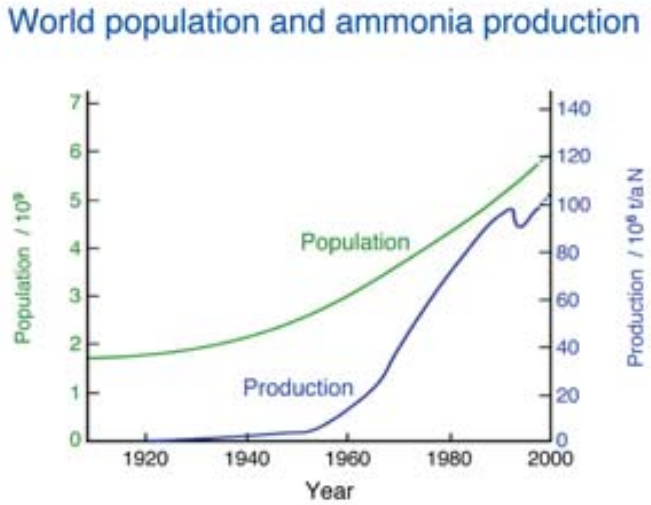
\includegraphics[width = 0.8 \textwidth]{figures/ammonia.png}
      \end{figure}  
      
    \column{0.45\textwidth}  
      \begin{block}{Umwelttechnik}
        \begin{itemize}
        \setlength{\itemindent}{-0.5em}
        \item Luftreinhaltung 
        \begin{itemize}
        \setlength{\itemindent}{-1.5em}
          \item Abgaskatalysatoren 
          \item Rauchgasentstickung 
        \end{itemize}
        \item Biokraftstoffe
        \begin{itemize}
        \setlength{\itemindent}{-1.5em}
          \item Fischer-Tropf-Synthese
        \end{itemize}
        \end{itemize}
      \end{block}
      
      \begin{columns}[t]
        \column{0.55\textwidth}
          \begin{figure}
            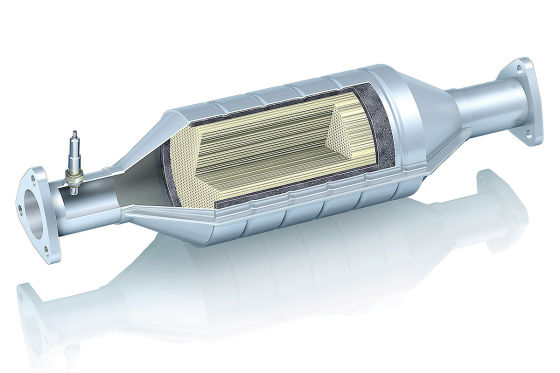
\includegraphics[width = 1.1 \textwidth]{figures/autokat.jpg}
          \end{figure}
        \column{0.5\textwidth}        
          \begin{figure}
            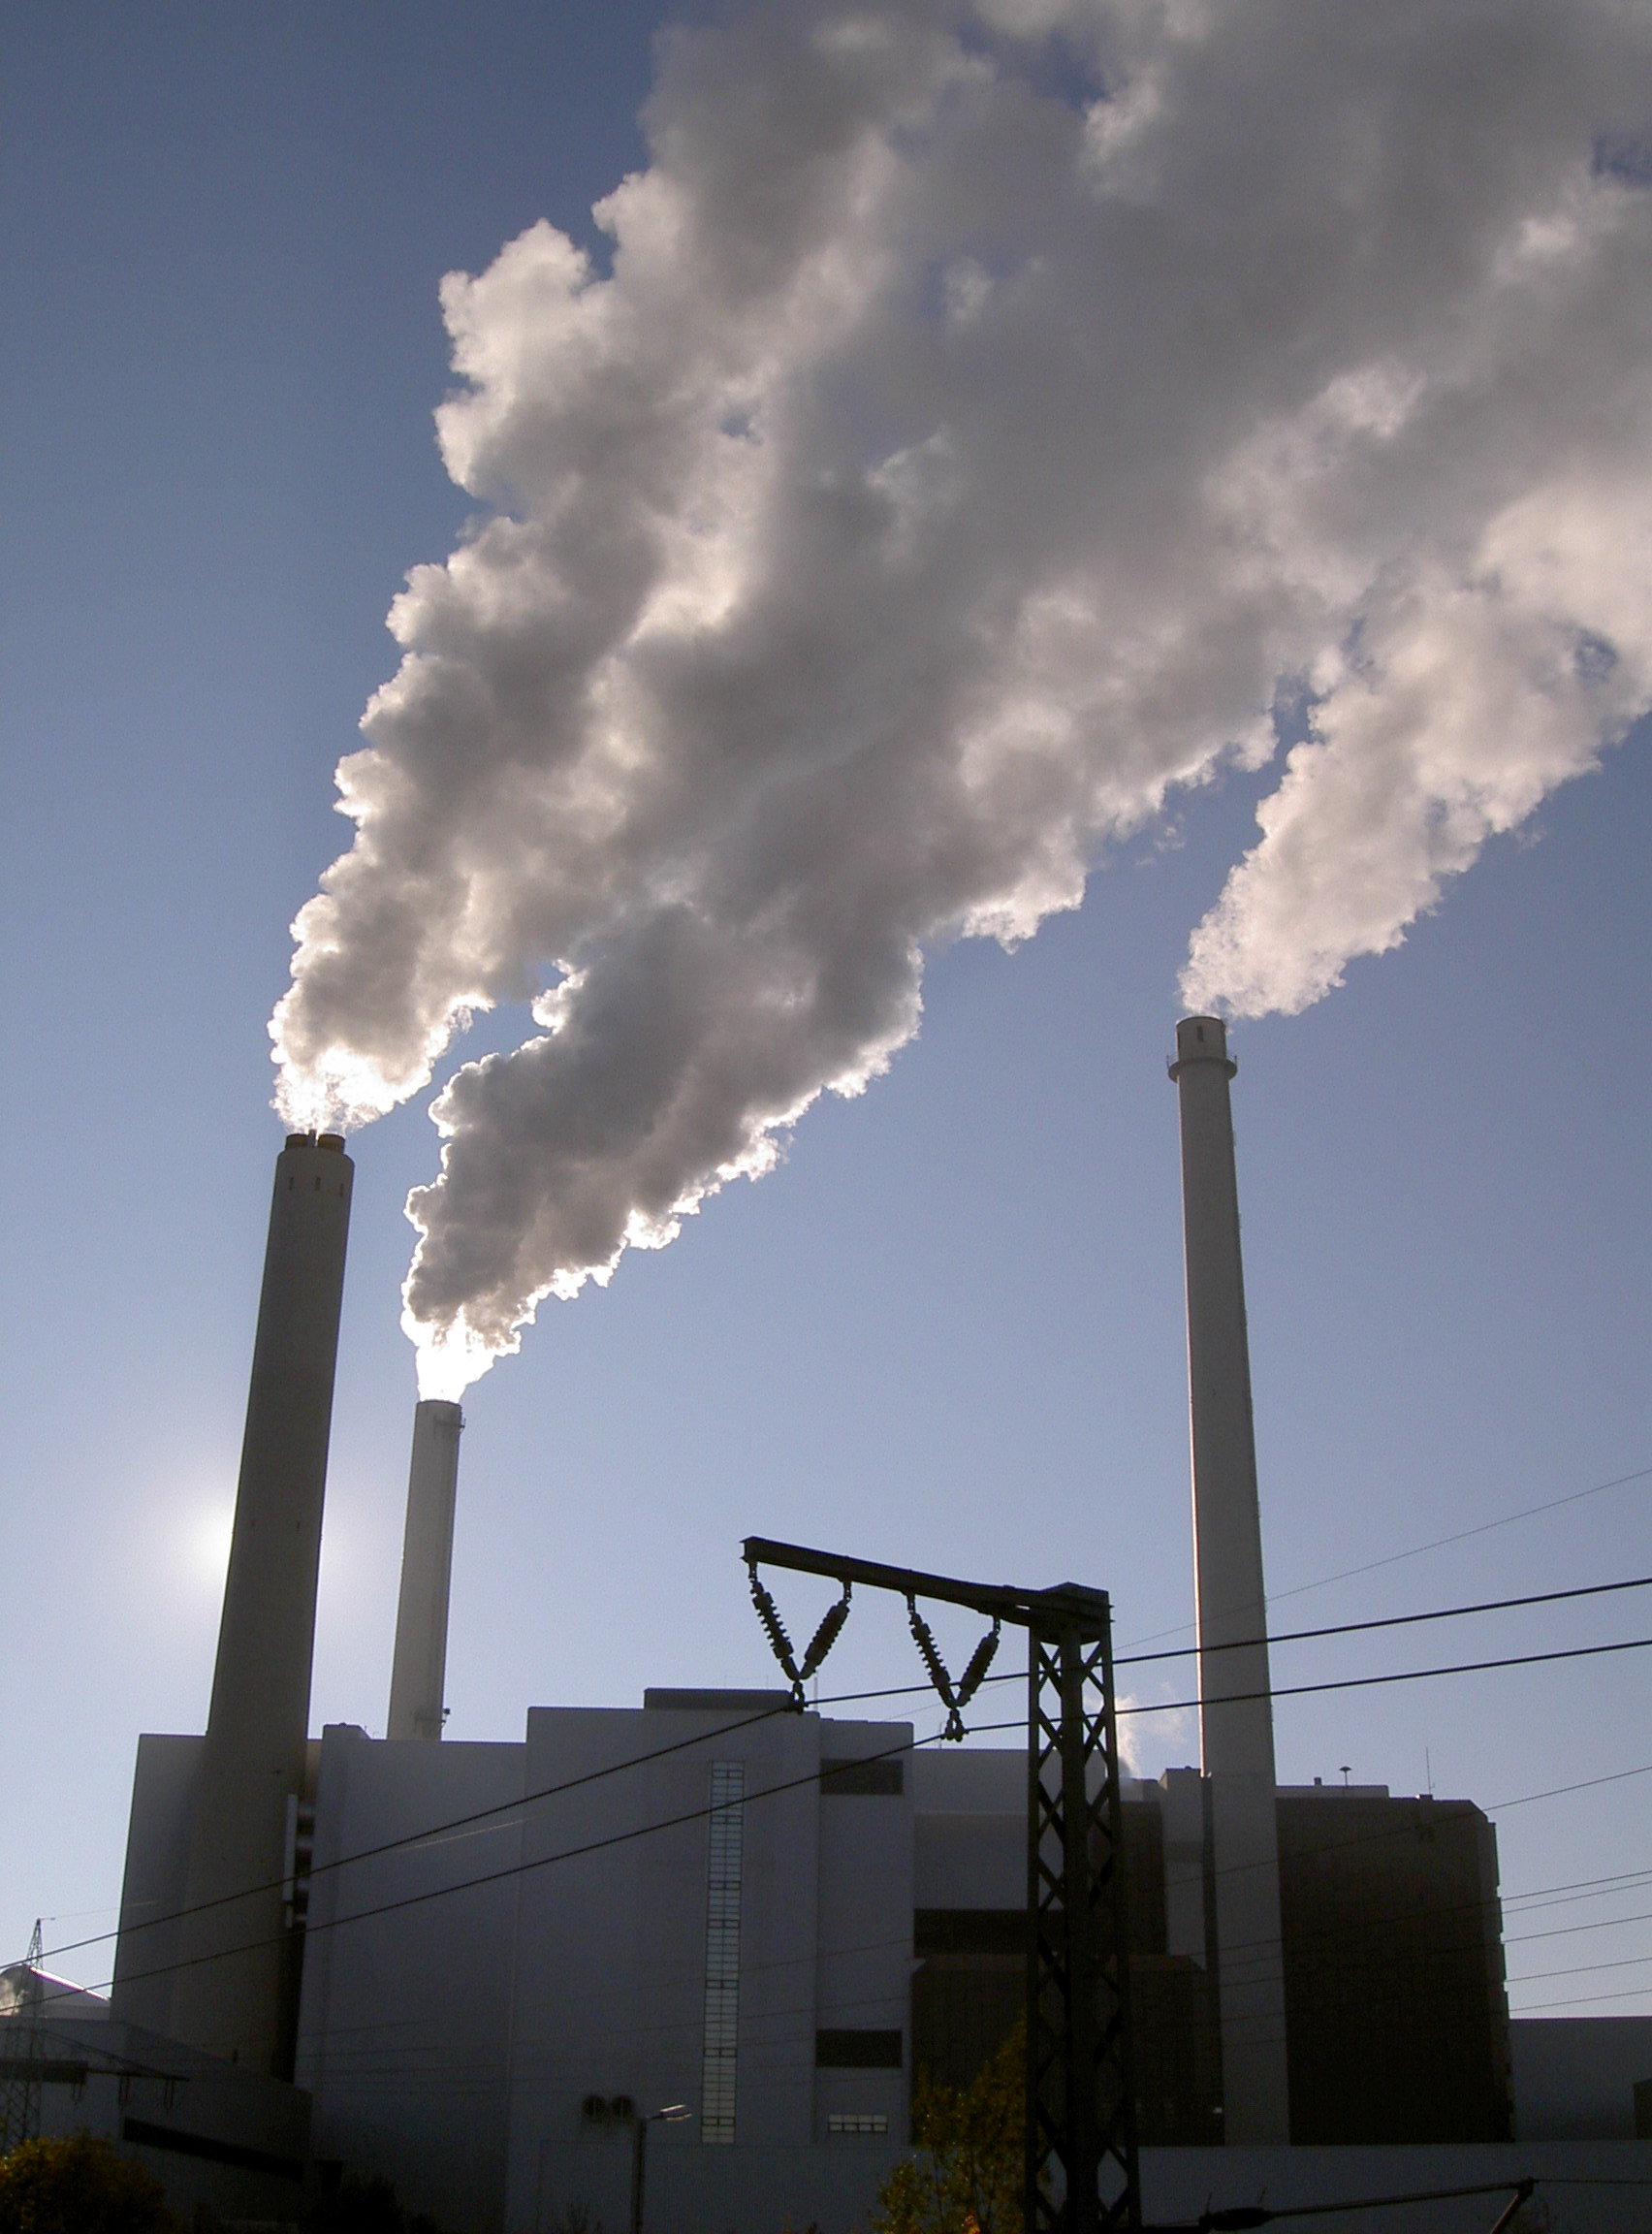
\includegraphics[width = 0.9 \textwidth]{figures/schornsteine.jpg}
          \end{figure}        
      \end{columns}
  \end{columns}
\end{frame}

\begin{frame}{}
 
\end{frame}



% \begin{frame}[plain]{Outline}
%   \tableofcontents
%   % Die Option [pausesections] k�nnte n�tzlich sein.
% \end{frame}



% Da dies ein Vorlage f�r beliebige Vortr�ge ist, lassen sich kaum
% allgemeine Regeln zur Strukturierung angeben. Da die Vorlage f�r
% einen Vortrag zwischen 15 und 45 Minuten gedacht ist, f�hrt man aber
% mit folgenden Regeln oft gut.  

% - Es sollte genau zwei oder drei Abschnitte geben (neben der
%   Zusammenfassung). 
% - *H�chstens* drei Unterabschnitte pro Abschnitt.
% - Pro Rahmen sollte man zwischen 30s und 2min reden. Es sollte also
%   15 bis 30 Rahmen geben.
% 
% 
\end{document}
